\chapter{State of the Art}
\label{chap:soa}

\section{The Artificial Intelligence Spectrum} \label{sec:the_ai_spectrum}
%%Referencias a los tipos de modelos y a los modelos hibridos que hay y a los estudios quasifilosoficos sobre por que unos pisan a otros, reemplazan a otros, mejoran a otros, etc.

\begin{figure*}
    \centering
    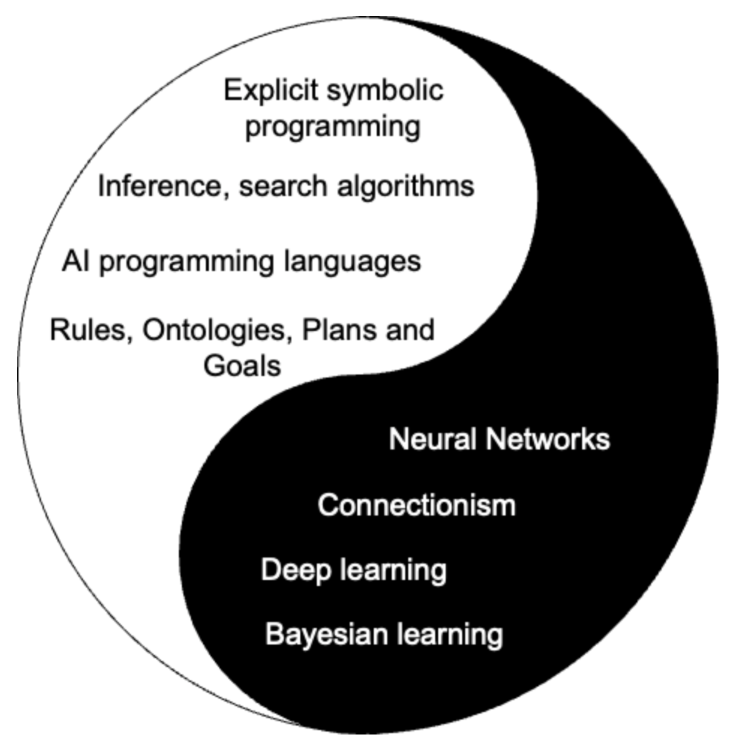
\includegraphics[width=.5\linewidth]{3_stateoftheart/figures/Lieberman_taxonomy.eps}
    \caption{AI Spectrum as depicted in \cite{lieberman_symbolic_nodate}}
    \label{fig:lieberman_tax}
\end{figure*}

Throughout the years, several categorizations have been proposed for the existing Artificial Intelligence (AI) models, each attending to a specific criterium. \cite{lieberman_symbolic_nodate} categorizes AI models considering their input in two categories: symbolic (also referred to as "classic AI") and subsymbolic. These two types are disjoint and complimentary to each other. \cite{lieberman_symbolic_nodate} depict the AI spectrum as a \textit{yin-yang} (Figure \ref{fig:lieberman_tax}), where the flaws of one kind are compensated by the benefits of the other. While this categorization presents a simple and general overview of the existing AI models, it lacks a middle ground where hybrid approaches can be categorized. 

Opposite to this vision, where the focus is on the input, \cite{loyola-gonzalez_black-box_2019} envisions the AI spectrum from the perspective of the output. This taxonomy categorizes AI approaches as \textit{white-box} or \textit{black-box} considering whether the process that lead to a given output can be explained or not. The notation \textit{black-box} is used to describe those models whose inference process cannot be explain, which mainly applies to machine learning models.  \textit{Black-box} models can be subsequently grouped in: hyperplane-based, neural networks, probability-based and instance-based. On the opposite side of this spectrum lie \textit{white-box} models, which relate to those approaches whose inference process can be understood and explained. Decision trees, rule-based systems, or fuzzy logic are encompassed in this category.


\begin{figure}
    \centering
    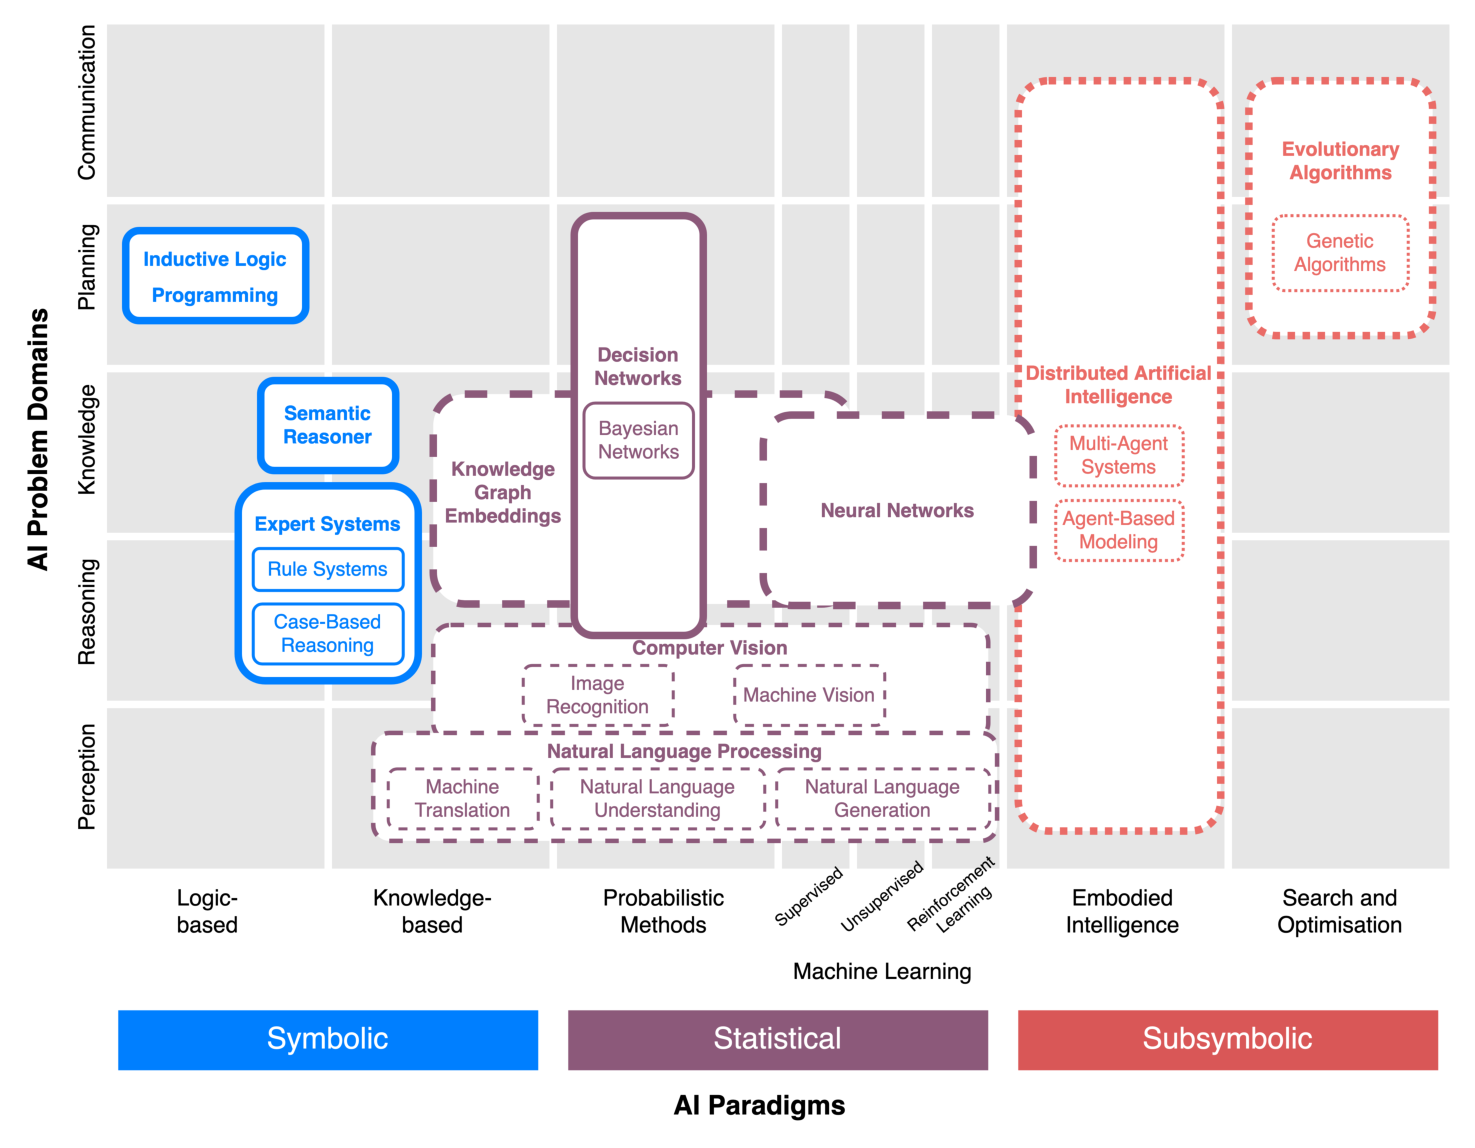
\includegraphics[width=\linewidth]{3_stateoftheart/figures/AI_Map.eps}
    \caption{Map of AI models combining the taxonomy of \cite{corea_ai_2019} with the taxonomy considered in this thesis. Symbolic, statistical and subsymbolic approaches are colour-coded in blue, purple and red respectively. Knowledge-based and computational intelligent systems are coded in continuous and non-continuous lines, respectively. Dashed lines depict deep learning approaches, while dotted lines depict other computational intelligent approaches.}
    \label{fig:ai_map}
\end{figure}


More recently, \cite{corea_ai_2019} proposed a two dimensional categorization of AI technologies. Instead of considering the input or output of the model, this taxonomy focuses on the application domains of each paradigm and its reasoning paradigm. Figure \ref{fig:ai_map} portrays this categorization, where the Y-axis comprises the existing problem domains, while the$\times$-axis encodes the three considered paradigms: symbolic, statistical and subsymbolic. While the taxonomy proposed by \cite{lieberman_symbolic_nodate} only considered the symbolic (blue) and subsymbolic (red) categories, \cite{corea_ai_2019} also considers the statistical (purple) models as an in-between group between the two complimentary groups. Moreover, finer-grained subcategories can be distinguished inside each of the three main paradigms:
\begin{itemize}
    \item \textbf{Symbolic models:} The term \textit{symbolic} describes AI paradigms that not only employ symbolic representations as input, but have an inference process that can be understood and explained by humans. Two finer grained types are identified inside this category: logic-based and knowledge-based.
    \item \textbf{Statistical models:} While the taxonomy proposed by \cite{lieberman_symbolic_nodate} only comprised symbolic and subsymbolic models, which are treated as analogous and complimentary kinds, this taxonomy distinguishes statistical models from purely subsymbolic models. These models employ mathematical tools for reasoning and can be subsequently divided into probabilistic and machine learning models.
    \item\textbf{Subsymbolic models:} According to this taxonomy, the term \textit{subsymbolic} refers to the absence of previous knowledge needed to function. Embodied intelligence models and search and optimisation models are grouped under this criterion.
\end{itemize}

The previous taxonomies provided categories that were fully disjoint and, therefore, each particular model needed to belong to exclusively one of the types. The taxonomy of \cite{corea_ai_2019} enables a higher degree of flexibility, as models can be applied under different problem domains as well as use different reasoning paradigms.
%%Taxonomias de la mas antigua a la mas moderna
\cite{hopgood_2009_knowledge-based} proposed a division of AI paradigms in two main categories: knowledge-based systems and computationally intelligent systems. Knowledge-based systems require explicit representations of knowledge in a symbolic form, while computationally intelligent systems use nature-inspired paradigms where no background knowledge is required to reason. This taxonomy can be merged with the taxonomy of \cite{corea_ai_2019}, providing a three-dimensional taxonomy as depicted in Figure \ref{fig:ai_map}. A third dimension depicts whether the paradigm can be classified as knowledge-based (continuous line) or computationally intelligent (discontinuous line). 

Deep Learning was introduced after \cite{hopgood_2009_knowledge-based}'s taxonomy was defined and is therefore not featured in this categorization. Therefore, a slight update on this base taxonomy is proposed to include deep learning models. Figure \ref{fig:ai_map} makes a distinction inside the computationally intelligent models, denoting with a dashed instead of a dotted line those paradigms that can be considered as deep learning. 

After combining the taxonomies presented in \cite{hopgood_2009_knowledge-based} and \cite{corea_ai_2019}, the final three-dimensional categorization of the models is as follows:
\begin{itemize}
    \item \textbf{Knowledge-Based Systems:} These systems fit almost perfectly the definition previously provided for the symbolic paradigms. Therefore, this category groups all the models that require from background expert knowledge to reason:
    \begin{itemize}
        \item \textit{Inductive Logic Programming (ILP):} This term was first introduced by \cite{Muggleton1991}, describing this field as "\textit{the area of AI which deals with the induction of hypothesised predicate definitions from examples and background knowledge}". ILP is one of the prime examples of symbolic learning, using fully expressive representations to encode logical clauses and knowledge, making the input, output and the induction process fully explainable.
        \item \textit{Semantic Reasoners:} Instead of expressing background knowledge by means of logical clauses or predicates as in ILP, semantic reasoners use ontologies to encode background knowledge. Ontologies \citep{noy2001ontology} provide explicit specifications of conceptualizations which are shared and understood between humans and machines. Moreover, ontologies present a formal definition of classes (or types) and the properties and relations between those classes and their instances in a given domain. From the information encoded in an ontology, a semantic reasoner (also referred to as the reasoning engine) can infer new axioms from the existing axioms.
        \item \textit{Expert Systems:} Formally, an expert system can be described as an AI system capable of emulating the decision-making process of a human expert of a given domain. These systems are composed by two differentiated parts: an inference engine and a knowledge base. The knowledge base encodes the facts, rules and background information needed. The inference engine applies the rules existing in the knowledge base to the known facts to infer new facts. \textit{Rule Systems} are the cornerstone of expert systems, using if-then clauses to infer new information from the already existing knowledge. As both facts and rules are encoded in a declarative way, the inference process can be fully understood and explained by humans. \elvitodo{A lo mejor esto hay que aumentarlo un poco}
        
        \textit{Case-Based Reasoning} (CBR) \citep{overview_cbr} is another example of an expert system. In this case, the knowledge base is replaced by a case base, where a set of problem-solution tuples (or cases) are stored. CBR implements a continuous cycle, where the model improves overtime by including the knowledge acquired from the resolution of new problems, whose solutions are then stored in the case base. Therefore, the performance of the model improves overtime. A CBR model is composed of four distinct phases: retrieve, reuse, revise and retain. When a new problem enters the system, the retrieve phase is triggered, returning the most similar existing cases to the introduced one. From the most similar cases, a tailored solution for the input problem is devised in the reuse stage using the already known solutions of the most similar cases. The proposed solution is then revised, determining whether it is suitable for the problem or not. If the solution satisfies the input problem, the newly generated case is stored in the case base, and will serve for the resolution of subsequent problems.   
    \end{itemize}
    \item \textbf{Computational Intelligence:} Following the taxonomy from \cite{hopgood_2009_knowledge-based}, computational intelligence models cover both statistical and subsymbolic paradigms. The remaining of the computational intelligence spectrum according to the proposed categorization comprises the following models:
    \begin{itemize}
        \item \textit{Decision Networks,} also referred to as influence diagrams \citep{poole_2017_ai_foundations} are graphical representations of a finite and sequential decision problem. A decision network is generally composed by three types of nodes: chance, decision and utility nodes, which are assorted as a directed cyclic graph. \textit{Bayesian Networks} \citep{friedman_1997_bayesian} are the most common paradigm amongst decision networks. Based on the Bayes theorem, these decision networks model the conditional dependencies between nodes, modelling the probability of each variable. Therefore, Bayesian networks can be used both to infer an outcome given the input variables as well as to determine the most feasible combination of variables that leads to an output. As variables are explicitly declared and their probabilities are known, the inference process of Bayesian networks can be also fully interpreted.
        \item \textit{Multi-Agent Systems} (MAS) \citep{Ferber:1999:MSI:520715} are one of the most extended paradigms for the simulation of scenarios involving complex entities. These models comprise a set of self-organized intelligent agents which cooperate and interact to perform a given task. As it involves several independent components, these models are capable of solving complex tasks that can not be solved by single-task systems. Agents of a MAS are autonomous, act locally, and are independent of each other. 
        \item \textit{Evolutionary Algorithms} \citep{GALVAN2003573} are heuristic-based systems inspired by natural evolution mechanisms. They are mostly applied to combinatorial problems, as they can greatly reduce the time required to go through the search space while still reaching an optimal solution. Typically, an evolutionary algorithm comprises four steps: initialization, selection, operation, and termination. These stages are closely related to those happening in natural selection. Therefore, those candidate solutions that better fit the problem will replicate and proliferate, while those inadequate will be slowly discarded throughout the evolution process. 
    \end{itemize}
    \item \textbf{Deep Learning} was first introduced in 2012 \citep{bengio_2012_dl_review}. This term was coined to describe the upcoming trend of computational intelligence models, especially neural networks, that are capable of reasoning at a very high level of abstraction. There is not a formal unified definition for the models encompassed in this trend, but they share common features such as requiring elevated computational resources, performing more than two in-between transformations between the input and the output (i.e: having more than two intermediate layers in neural networks) or learning multiple representations with different abstraction levels.
    \begin{itemize}
        \item \textit{Neural Networks}, are connected systems inspired by the neurological behaviour of brains \citep{Rosenblatt58theperceptron:}. These models are composed by the interconnection of single processing units called 'neurons', capable of performing simple mathematical operations. A neural network receives an input, which is subsequently processed by the neurons to generate an output value. In order for the output value to be coherent with the input, the neural network requires a training (or learning) process, where the weights of the connections between the neurons are learned using the error gradient backpropagation from a loss function \citep{rumelhart_1987_backpropagation}.  
        
        % Three main types of neural network learning can be distinguished: supervised, unsupervised and reinforcement learning. In \textit{supervised learning}, a set of known inputs with their corresponding outputs 
        \item \textit{Computer Vision} is one of the primary fields of application of deep learning. This area encompasses methods capable of capturing, processing, analyze and reason over graphic data. Convolutional Neural Networks (or CNNs) have been the dominant paradigm of this area since 2012 \citep{alexnet}, reaching state-of-the-art results in most computer vision tasks.
        
        \item \textit{Natural Language Processing} (or NLP) \citep{chowdhury_2003_nlp} encompasses those models and tasks focusing on understanding, processing, and generating spoken and written words similarly to humans. While knowledge-based systems were previously predominant in the area, the existing models have been slowly replaced by a series of neural network architectures capable of performing the same tasks with remarkably better results. Some neural network architectures specific of this area include \textit{Bidirectional Long-Short Term Memories} (Bi-LSTM)\citep{devlin-etal-2019-bert,peters-etal-2018-deep} and \textit{Recurrent Neural Networks} (RNNs) \citep{wang-etal-2016-combination}. 
        
        \item \textit{Knowledge Graph Embeddings} \citep{dai_survey_2020} aim to arithmetically represent the information encoded in the facts contained in a knowledge graph, associating every entity and relation with a unique representation. The resulting depiction aims to embed the knowledge stored in the facts so that several constraints are met. One of the most important restrictions is that those entities representing similar concepts should have similar embeddings, meaning that the distance between their representations should be fairly small. According to the scoring function, two different types of approaches can be defined: translation-based and semantic matching models. Translation-based models aim to minimize distance-based scoring functions, while semantic matching models measure the plausibility of a given fact by matching the latent semantics of entities and relations.
    \end{itemize}

\end{itemize}

%%Nuestra taxonomia y cuales son cada uno 

% \section{Design Methods for Hybrid Learning Systems}
\section{Neurosymbolic Systems}
While the taxonomies in Section \ref{sec:the_ai_spectrum} presented some differences amongst them, they all share a common ground: categorizing the 
AI models into analogical and complimentary aggregations. \textit{Neurosymbolic} (or hybrid learning) AI describes a set of proposed methods designed to integrate analogous AI models, generating new approaches that combine the benefits of both models under a unified framework. As \cite{valiant_three_2003} claimed: \textit{"The aim is to identify a way of looking at and manipulating commonsense knowledge that is consistent with and can support what we consider to be the two most fundamental aspects of intelligent cognitive behaviour: the ability to learn from experience and the ability to reason from what has been learned"}. Several efforts have been conducted on this direction, proposing strategies, categorizations, and studying the limitations of this integration. 

\subsection{Motivation}
%%Papers referentes a por qué, limitaciones, etc. Aquí va el paper de sensors
\cite{mcgarry_hybrid_1999} theorized about the potential benefits of combining symbolic and subsymbolic systems, represented by rule-based systems and neural networks, respectively. According to \cite{mcgarry_hybrid_1999}: "\textit{The ability of neural networks to perform tasks that would otherwise prove difficult or intractable to symbolic computing systems is now recognized}". This statement clearly illustrates the core idea behind neurosymbolic systems: combining the benefits of symbolic and subsymbolic models such that the resulting hybrid system enables the solution of tasks that can not be solved by just one of the kinds. 

% This statement has been subsequently validated by various works throughout the years, such as \cite{mira_neurosymbolic_2004}, \cite{bader_dimensions_2005} or \cite{garcez_neural-symbolic_2019}.

\begin{table}
\centering
\caption{Application domain and assessment of the works employing predictive techniques over knowledge bases. 
%Define if appropriate
The metrics reported in the table are: M1 (scalability), M2 (interpretability), M3 (generalization capability), M4 (low resource consumption) and M5 (knowledge base exploitation). The degree of fulfilment of each metric per resource is indicated as follows:$\times$ = yes/high, / = partly/medium, empty = no/low. Symbolic and subsymbolic approaches are depicted in green and red respectively. \label{tab:sensors_reasoning}}
\resizebox{.75\linewidth}{!}{
%\begin{tabular}{C{3.5cm}C{2.5cm}C{3.5cm}C{2.5cm}C{2.5cm}C{1cm}C{1cm}C{1cm}C{1cm}}
\begin{tabular}{M{3.5cm}M{2.2cm}M{4cm}M{.5cm}M{.5cm}M{.5cm}M{.5cm}M{.5cm}M{1.5cm}}
\toprule
{\textbf{Resource}} &
{\textbf{Domain}} &
\textbf{Predictive} \textbf{Technique} &
{\textbf{M1}} &
{\textbf{M2}} &
\textbf{M3} &
\textbf{M4} &
\textbf{M5} &
\textbf{Score} \\
\midrule
\rowcolor{teagreen}\cite{aliandlee}         & \textit{Health}                   & \textit{Rules Manually Created by Experts}                           &                      &$\times$                         &                                 &$\times$                                 &$\times$                        & 3                      \\
\rowcolor{teagreen}\cite{barnwaletal}      & \textit{Risk/Resource Management} & \textit{Probabilistic distributions}                                 &                      &$\times$                         &                                 &$\times$                                 &$\times$                        & 3                      \\ 
\rowcolor{tearose}\cite{bogaleetal}       & \textit{Multidomain}              & \textit{Multivariate Linear Regression}                              & /                    & /                         & /                               &$\times$                                 &$\times$                        & 3.5                    \\ 
\rowcolor{tearose}\cite{chungetal2018}        & \textit{Health}                   & \textit{Deep Neural Network}                                         &$\times$                    &                           &$\times$                               &                                   &$\times$                        & 3                      \\
\rowcolor{tearose}\cite{dimitrovetal}     & \textit{Housing}                  & \textit{Bayesian Network} \citep{bayesiannetwork}                                             &                      &$\times$                         &                                 &$\times$                                 &$\times$                        & 3                      \\ 
\rowcolor{teagreen}\cite{duyenandnhon}      & \textit{Education}                & \textit{If-then manually created rules}                              &                      &$\times$                         &                                 &$\times$                                 &$\times$                        & 3                      \\ 
\rowcolor{tearose}\cite{fastetal}         & \textit{Housing}                  & \textit{Word2Vec vector generation + cosine distance comparison}     &$\times$                    &$\times$                         &$\times$                               & /                                 &$\times$                        & 4.5                    \\ 
\rowcolor{tearose}\cite{haoetal}          & \textit{Housing}                  & \textit{Half-Duplex Search algorithm}                                &                      &$\times$                         &                                 &$\times$                                 &$\times$                        & 3                      \\ 
\rowcolor{tearose}\cite{kimandchung}       & \textit{Health}                   & \textit{Neural Network}                                              &$\times$                    &                           &$\times$                               & /                                 &                          & 2.5                    \\ 
\rowcolor{teagreen}\cite{KimandChang}       & \textit{Health}                   & \textit{Pearson's correlation coefficient + Collaborative Filtering} \citep{pearsoncorrelation,collaborativefiltering,collaborativefiltering2} &                      &$\times$                         &                                 &$\times$                                 &$\times$                        & 3                      \\ 
\rowcolor{tearose}\cite{machadoetal}      & \textit{Housing}                  & \textit{Multi-entity Bayesian Networks} \citep{mebn}                              &                      &$\times$                         &                                 & /                                 &$\times$                        & 2.5                    \\ 
\rowcolor{teagreen}\cite{Martinruizetal}  & \textit{Health}                   & \textit{Rules manually created by experts}                           &                      &$\times$                         &                                 &$\times$                                 &$\times$                        & 3                      \\ 
\rowcolor{teagreen}\cite{olszewskiturek} & \textit{Mobility}                 & \textit{CART Trees} \citep{carttrees}                                                   & /                    &$\times$                         &$\times$                               &$\times$                                 &$\times$                        & 4.5                    \\
\rowcolor{teagreen}\cite{Olzewskietal}    & \textit{Government}               & \textit{Fuzzy logical rules} \citep{fuzzyenvironment}                                         &                      &$\times$                         & /                               &$\times$                                 &$\times$                        & 3.5                    \\ 
\rowcolor{teagreen}\cite{orlowskietal}     & \textit{Mobility}                 & \textit{Fuzzy logical rules}                                         &                      &$\times$                         & /                               &$\times$                                 &$\times$                        & 3.5                    \\ 
\rowcolor{teagreen}\cite{peraletal}        & \textit{Health}                   & \textit{C4.5 Tree} \citep{c45tree}                                                   &                      &$\times$                         &                                 &$\times$                                 & /                        & 2.5                    \\ 
\rowcolor{tearose}\cite{persaudetal}      & \textit{Mobility}                 & \textit{Deep Neural Network}                                         &$\times$                    &                           &$\times$                               &                                   & /                        & 2.5                    \\ 
\rowcolor{tearose}\cite{ribonietal}       & \textit{Health}                   & \textit{Random Forest} \citep{randomforest}                                               &$\times$                    & /                         &$\times$                               & /                                 &$\times$                        & 4                      \\ 
\rowcolor{tearose}\cite{siimobility-parking,siimobility-consult,siimobility-journal}        & \textit{Mobility}                 & \textit{Bayesian Regression ANNs} \citep{brann1,brann2,brann3}                                     &$\times$                    & /                         &$\times$                               & /                                 &$\times$                        & 4                      \\
\rowcolor{teagreen}\cite{xuandli}           & \textit{Risk/Resource Management} & \textit{Fuzzy logical rules}                                         &                      &$\times$                         & /                               &$\times$                                 &$\times$                        & 3.5                    \\ 
\rowcolor{teagreen}\cite{zavalaetal}       & \textit{Mobility}                 & \textit{RIPPER rules} \citep{ripper}                                                &                      &$\times$                         &                                 &$\times$                                 &$\times$                        & 3                      \\ \bottomrule

\end{tabular}
}
\end{table}
To further explore the existence, limitations, and causes of the application of neurosymbolic models, a systematic review was conducted in the context of ambient intelligence. This work is extensively presented in \cite{amador_systematic_review_2019}, and it is part of the contributions of this thesis. The conducted review studies the interactions between knowledge bases and machine learning models, as well as their specific applications. Different application subdomains were identified to clearly identify the scope of application of each proposal. This finer-grained analysis enables a better comprehension of the reasons why a certain model is chosen for a certain task. The identified subdomains, following the categorization proposed by \cite{ahmedetal} are: health, housing, education, mobility, risk and resource management, government, and multidomain. Another main goal of this study is to assess whether and how background knowledge (in the form of a knowledge base) is integrated into different predictive and decision-making models.

In the studied resources, background knowledge was mostly extracted from three sources: data provided by users, previously existing KBs, and sensor data, being the latest the most prominent one. Regarding the role of the KB, it varies greatly across the different subdomains. In the health, mobility, risk and resource management and housing domains, the KB is built with the purpose of subsequently feeding a predictive model, doting it with background knowledge and enhancing its reasoning capabilities. This statement does not hold in the government and education domains, where the KB plays the primary role instead of serving as a secondary element.

The following metrics (which relate to the expected features of neurosymbolic systems) were evaluated to study the different proposals in which the KB is integrated within the predictive model: scalability, interpretability, generalization ability, resource consumption, and relevance of the knowledge base to the predicting process. Table \ref{tab:sensors_reasoning} summarizes the findings of this study. Despite the heterogeneity between proposals, it is worth noticing that the majority of the employed paradigms are symbolic (green highlighted rows), thus scoring high in interpretability (M2). In the work of \cite{olszewskiturek} a neural network is also evaluated on the task, outperforming other approaches. The authors, however, decide on a decision tree as their final model, stating that even when its performance was subpar with respect to the neural network, they preferred to employ a model that was interpretable. This decision is quite remarkable, as it clearly showcases one of the biggest breaches between symbolic and subsymbolic models: the lack of explainability. 

Moreover, all proposals used the KB when building the predictive model, thus successfully integrating background knowledge. It is also worth noticing that, for subsymbolic approaches (red coloured rows), there exists a direct relation between scalability (M1) and generalization capability (M3), featuring simultaneously on several resources. This does not apply to purely symbolic models, where these features are ranked either as partial or null. 

Therefore, this study served to further evidence the existing chasm between symbolic and subsymbolic approaches, evidencing the necessity of middle-ground solutions that combine the positive features of both types.

%Después de nuestra referencia, el resto

\subsection{Design}
%Papers de boxología
\cite{mcgarry_hybrid_1999} is one of the first works to draw the limitations of neurosymbolic models, focusing on the integration of neural networks and rule-based systems. According to this work, the key features a neurosymbolic system should present are: i) the ability to reason with noisy and incomplete data, ii) learning incrementally from new experience, iii) generalize and explain the chain of reasoning. %%LUEGO ESTO SE EXTIENDE

\begin{figure}
    \centering
    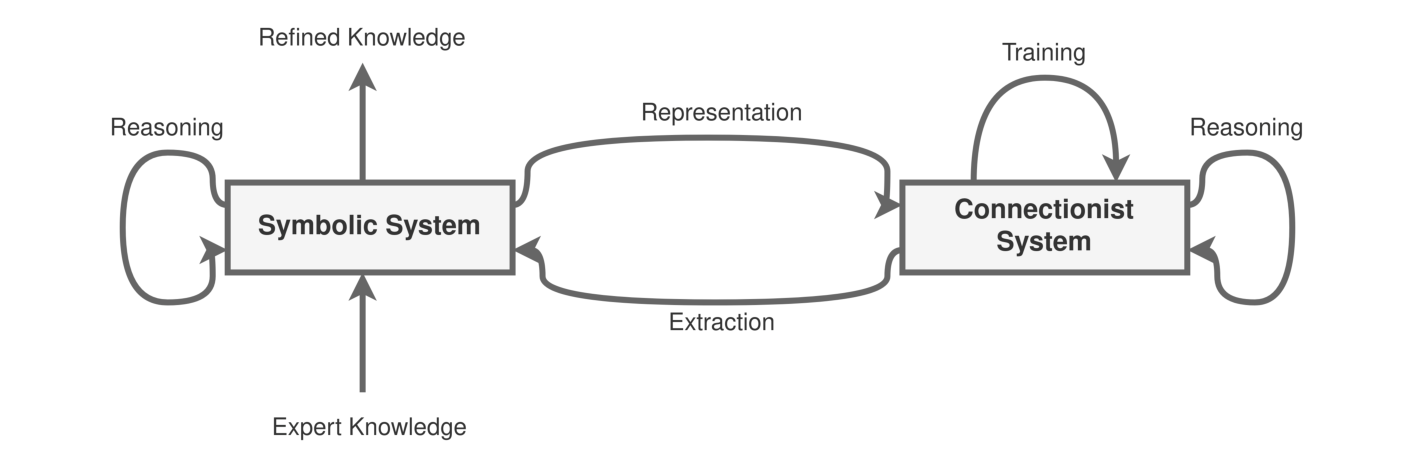
\includegraphics[width=\linewidth]{3_stateoftheart/figures/Neurosymbolic_Bader.eps}
    \caption{Neurosymbolic learning cycle. Extracted from \cite{bader_dimensions_2005}}
    \label{fig:neuro_cycle}
\end{figure}

This idea was further expanded by \cite{bader_dimensions_2005}, which introduced neurosymbolic learning as a continuous cycle. Figure \ref{fig:neuro_cycle} illustrates this idea, where interactions between the symbolic and subsymbolic systems do not occur in a linear way, but in a close cycle composed by individual interactions between both. For example, the symbolic system could play the role of a front-end, where expert knowledge is collected. This knowledge could then be encoded into the subsymbolic system during the training process, providing additional information that may not be inferred otherwise by the model. Moreover, the knowledge acquired throughout the training process could be extracted, decoded, and introduced back to the symbolic system, introducing new patterns of restrictions that may not have been previously declared. This cyclical conception of neurosymbolic systems meets the features proposed by \cite{mcgarry_hybrid_1999}.

\cite{mira_neurosymbolic_2004} roots the creation of neurosymbolic models on two criteria: purpose and design. For the first criterion, the authors determine that neurosymbolic integration is required in those scenarios where neither all knowledge or data are available. Regarding the design of the system, two strategies are proposed:
\begin{itemize}
    \item \textit{Unification}, where the needs of both symbolic and subsymbolic models are merged into a single component. This design induces a certain level of explainability to the connectionist models, while still retraining their topology and learning capabilities.
    
    % Two different design paths are proposed for this: i) extending the computational capabilities of the connectionist models to include symbolic forms of representation and ii) reducing the grain size of the symbolic model to enable subsymbolic representation. These two paths converge to the replacement of connectionist local functions by parametric rules. 
    \item \textit{Hybridation}, where the symbolic and connectionist modules are interconnected. In this design, connectionist components serve as a supporting element to the main symbolic processor.
\end{itemize}

With the renewed interest in neurosymbolic computing in recent times, new proposals have emerged addressing the newly existing challenges in neurosymbolic computing. \cite{besold_neural-symbolic_2017} enunciated a set of principles for neurosymbolic integration. This work highlights one of the core elements of neurosymbolic models: the distinction between representation and reasoning. Typically, symbolic models play the representation role, while subsymbolic models are used for reasoning. Equal to \cite{bader_dimensions_2005}, \cite{besold_neural-symbolic_2017} envisions neurosymbolic integration like a cycle, comprising the following steps: i) translation of symbolic background knowledge to a subsymbolic representation, ii) training the subsymbolic model to extract general patterns about the data, iii) reason over new data using the subsymbolic model and iv) extract symbolic knowledge from the subsymbolic model. The final step not only provides explanation of the inference process, but facilitates transfer learning over the subsymbolic model.

\begin{figure}[h]
    \centering
    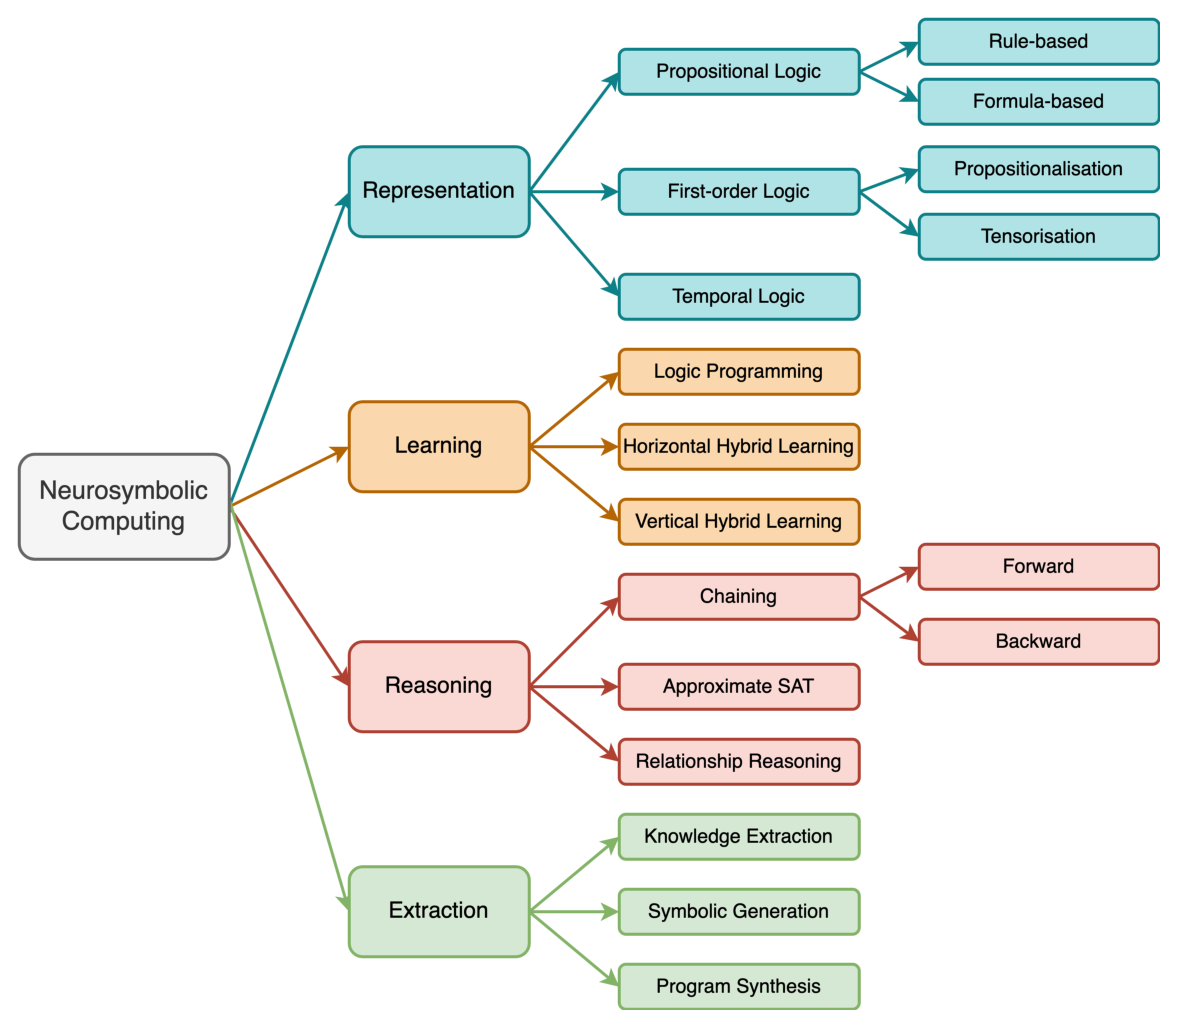
\includegraphics[width=.9\linewidth]{3_stateoftheart/figures/garcez_design.eps}
    \caption{Design dimensions proposed by \cite{garcez_neural-symbolic_2019}}
    \label{fig:garcez_design}
\end{figure}

More recently, \cite{garcez_neural-symbolic_2019} proposed a methodology for neurosymbolic integration that focuses on four key features: representation, extraction, reasoning, and learning. Figure \ref{fig:garcez_design} depicts the different design dimensions per feature. This methodology is compatible with the cyclic neurosymbolic learning process depicted in \cite{bader_dimensions_2005} and \cite{besold_neural-symbolic_2017}, but addresses additional features that were not previously considered and that are key to define neurosymbolic models.

In a recent work, \cite{garcez_neurosymbolic_2020} state that there always exist at least two options for designing a neurosymbolic model. In the first option, symbolic representations are translated and fed into a connectionist system, using the connectionist system to perform reasoning. In the second option, both the symbolic and connectionist models interact to perform reasoning. \elvitodo{Ampliar(?)}


%Regarding representation, \cite{garcez_neural-symbolic_2019} distinguishes three main groups: rule-based, formula-based, and embedding-based. In rule-based representation, the goal is to tailor the design of the connectionist system to mimic the representation of a rule system. Formula-based representations focus on mapping logical formulas to connectionist models. Finally, embedding-based representation projects symbolic representations into a continuous vector space, such that they can serve as input for a connectionist model. 

Some works focus on the visual representation of neurosymbolic systems via design patterns. \cite{harmelen_boxology_2019} introduces a boxology of design patterns for neurosymbolic systems. This work introduces a simple notation, composed by two types of representation techniques (data and symbolic) and two types of reasoning models (knowledge-reasoning and machine learning). This notation, while simple, is enough to represent any neurosymbolic system from a high-level perspective. \cite{van_bekkum_modular_2021} proposed an extension of this representation, providing a collection of compositional patterns with a higher specificity degree. This design methodology extends the two existing elements in the previous taxonomy with two additional types: processes and actors. In this design, \textit{processes} are used to describe operations that are performed outside the reasoning model, such as data transformation or instance generation. \textit{Actors} describe those autonomous elements that are external to the model but actively interact with the neurosymbolic system, such as humans, external apps or sensors.

%%Modelos hibridos, por que se reemplazan unos a otros, beneficios, aproximaciones, clasificaciones dentro de este marco. 

\subsection{Categorization}
The neurosymbolic classification framework proposed by \cite{medsker2020models} is one of the first efforts of categorizing neurosymbolic hybrid models under a unified framework. Five integration strategies are defined from a practical point of view based on the interaction degree, from fully independent to fully integrated: stand-alone, transformational, loose coupling, tight coupling, and fully integrated. This categorization does not model the input and output representations employed by each category, as well as the order in which the symbolic and connectionist modules are arranged.

\begin{figure}[t]
    \centering
    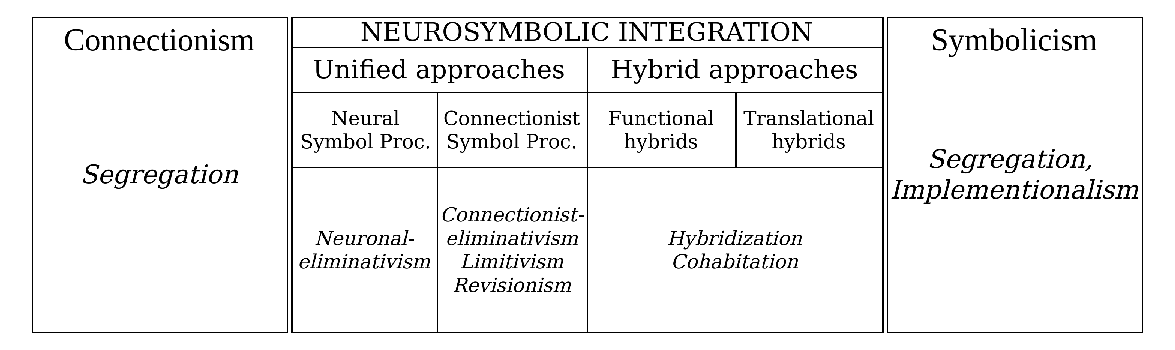
\includegraphics[width=\linewidth]{3_stateoftheart/figures/Hilario_categorization.eps}
    \caption{Synoptic view of neural, symbolic and neurosymbolic approaches. Extracted from \cite{hilario_overview_nodate}}
    \label{fig:hilario_categorization}
\end{figure}

\cite{hilario_overview_nodate} proposed a finer-grained categorization for neurosymbolic models, as depicted in Figure \ref{fig:hilario_categorization}. This work posed a distinction between the two main strategies of neurosymbolic integration: unification and hybridation. Unified systems are built on the idea that symbolic structures and processes are not strictly required and can emerge from their neural counterparts. On the contrary, hybrid systems are based on the synergistic combination of neural and symbolic models, leading to systems with enhanced cognitive and computational capabilities. Amongst the unified systems, \cite{hilario_overview_nodate} distinguishes between \textit{neuronal symbol processing} (NSP) and \textit{connectionist symbol processing} (CSP). While NSP aims to model the brain's high level functions emulating the behaviour of a real biological neuron, CSP is built for a specific task, commonly using artificial neural networks. Regarding hybrid strategies, they can be further categorized in functional and translational. Translational hybrids serve as a bridging element between unified models and functional hybrids, using symbolic structures with connectionist processors, but removing the need for a symbolic processor. Functional hybrids comprise complete symbolic and connectionist elements, combining neural networks with both symbolic structures and their processing elements. They can further be divided into loose and tight according to the degree of coupling between the symbolic and connectionist processors. 

%\begin{figure}
%    \centering
%    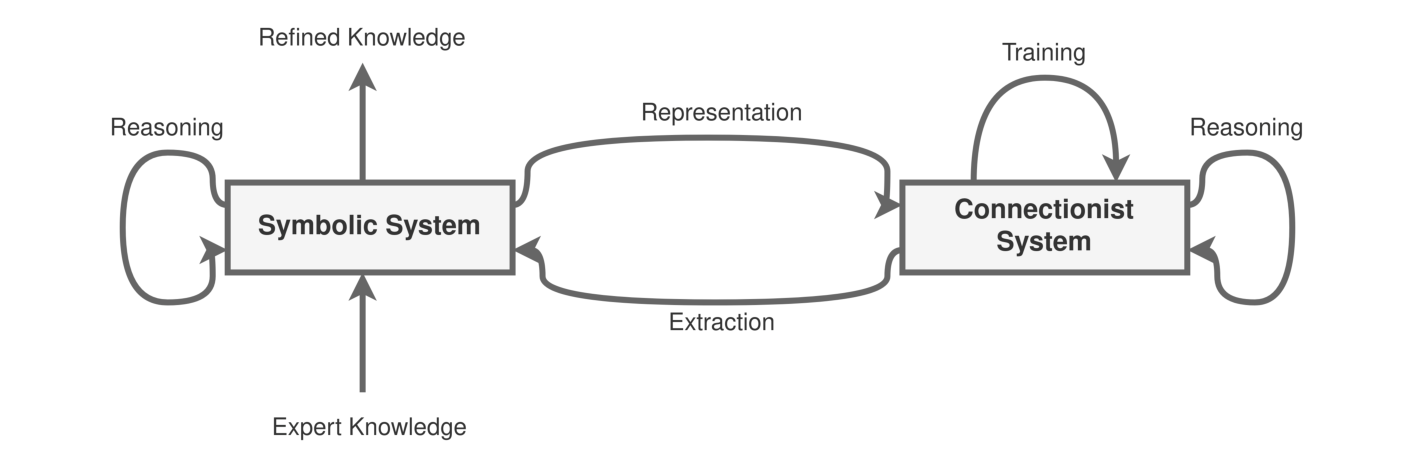
\includegraphics[width=\linewidth]{3_stateoftheart/figures/Neurosymbolic_Bader.eps}
%    \caption{Neural-symbolic learning cycle. Extracted from \cite{bader_dimensions_2005}}
%    \label{fig:bader_neurosymbolic}
%\end{figure}

\cite{mcgarry_hybrid_1999} focused on the categorization of a specific type of neurosymbolic models comprised by neural networks and rule-based systems. This categorization describes three integration types: \begin{itemize}
    \item \textit{Unified systems} implement a symbolic reasoning processing using subsymbolic elements, motivated by the idea that certain types of rule-based inference can be performed by subsymbolic models. The main limitation of these systems is their lack of scalability, as they rely on a symbolic-like representation paradigm.
    \item \textit{Translational systems} transform an initial symbolic representation into a subsymbolic one and viceversa. This bidirectional transformation enables, for example, the extraction of rules from neural networks, as well as the introduction of explicit background knowledge into the network. 
    \item \textit{Modular systems} are the most common type, integrating different individual modules (both symbolic and subsymbolic) under a unified framework.
\end{itemize} 

The categorization by \cite{hilario_overview_nodate} was later updated by \cite{bader_dimensions_2005}, proposing a more robust schema comprising three different dimensions. Instead of considering neurosymbolic integration as linear phenomena, \cite{bader_dimensions_2005} consider this process as a cycle. In this cycle, the symbolic system serves as an input point where expert knowledge can be collected, to be then fed into a connectionist system that can benefit from this background knowledge during the training process. Similarly, the knowledge acquired by the connectionist system after training can be returned to the symbolic system for further usage.

This conception of neurosymbolic integration enables a higher degree of flexibility than the previous categorizations. Subsequently, the categorization proposed by \cite{bader_dimensions_2005} provides a three-dimensional space, where each dimension has different degrees of flexibility. The categorization proposed in \cite{hilario_overview_nodate}, where models range from unified to translational, is treated as just one dimension in this categorization. This dimension is referred to as \textit{interrelation} in this categorization. The second dimension refers to the \textit{language}, which relates to the way in which the knowledge is encoded in the system. The third and final dimension encodes the \textit{usage} of the system.

%%Patrones de diseño con boxologia
\section{Deep Learning and Knowledge-Based Systems Integration} \label{sec:dl_kb_intregration_rw}

As discussed in the previous Section, several strategies can be followed regarding neurosymbolic system design. All these strategies, however, can be grouped in two main trends: integration and extraction. Integration approaches aim to combine symbolic and subsymbolic models under a unified framework to perform a certain task. In \cite{van_bekkum_modular_2021} several compositional integrative patterns are described, covering an extended set of tasks. 
\begin{figure}[t]
  \centering
  \begin{tabular}{@{}c@{}}
    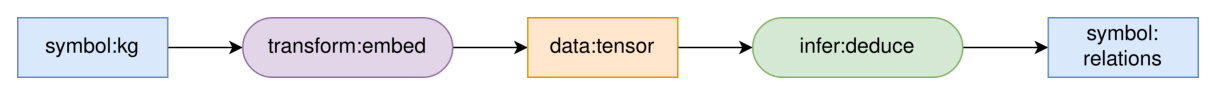
\includegraphics[width=.9\linewidth]{3_stateoftheart/figures/vanBekkum_LinkPrediction.eps} \\[\abovecaptionskip]
    \small (a) Knowledge Graph Embedding 
  \end{tabular}

  \vspace{\floatsep}

  \begin{tabular}{@{}c@{}}
    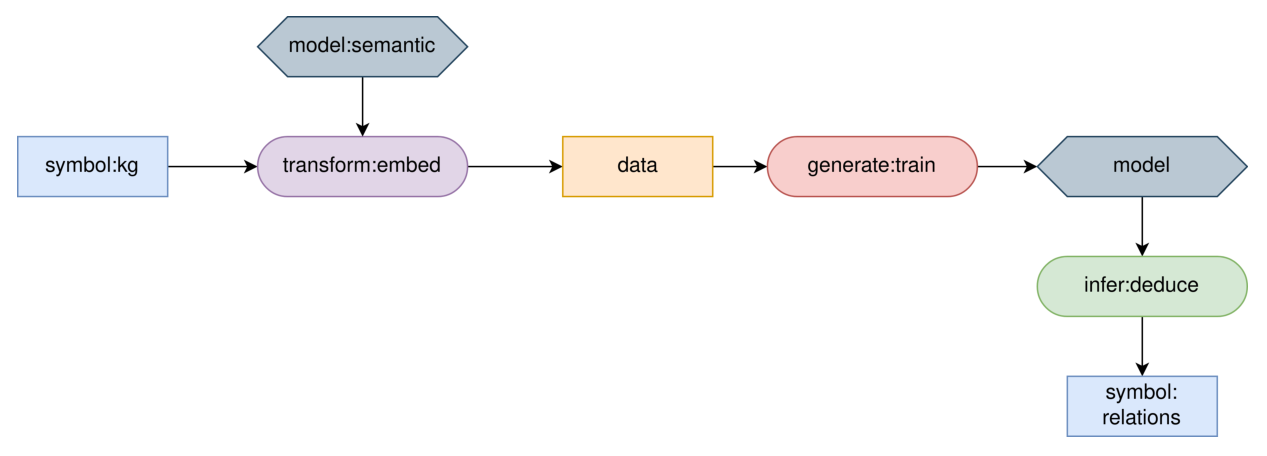
\includegraphics[width=.9\linewidth]{3_stateoftheart/figures/vanBekkum_GNN.eps} \\[\abovecaptionskip]
    \small (b) Graph Neural Network
  \end{tabular}

  \caption{Design pattern of two models for Knowledge Graph Completion according to \cite{van_bekkum_modular_2021}}\label{fig:van_bekkum_kgc}
  
  \extralabel{fig:van_bekkum_kgc_kge}{(a)}
  \extralabel{fig:van_bekkum_kgc_gnn}{(b)}
\end{figure}

Knowledge Graph Completion (KGC) \citep{nickel_review_ml_kg_2016,wang_kge_survey_2017} is one of the scenarios comprised in the collection. Knowledge Graphs (KGs) are composed by three elements: a set of entities $\mathcal{E}$, a set of relations $\mathcal{R}$, and the interactions between entities and relations, denoted as \textit{facts} or triples. Facts follow the fixed structure $(s,p,o)$, where $s$ and $o$ are the \textit{subject} and \textit{object} entities respectively, and $p$ is the \textit{predicate} that connects them. KGC aims to mine new facts from the existing KG information. Two main subtasks can be identified within KGC: link prediction and triple classification. In triple classification, the goal is to determine whether a potential fact $(s',p',o')$ is feasible or not. In link prediction, given an incomplete fact $(?,p,o)$ or $(s,p,?)$, the goal is to find the remaining element that maximizes the feasibility of the fact. 

\elvitodo{ARREGLAR REFERENCIAS}



Figure \ref{fig:van_bekkum_kgc} depicts the design patterns (according to \cite{van_bekkum_modular_2021}) of the two main approaches for KGC. Figure \ref{fig:van_bekkum_kgc_kge} depicts the general pattern of a Knowledge Graph Embedding model for KGC. These neurosymbolic models follow a straightforward approach, where the symbolic input (KG) is converted into a tensor representation with a embedding operation. This subsymbolic representation can then be used to infer new facts, which can be then decoded back to a symbolic format. Graph Neural Networks (Figure \ref{fig:van_bekkum_kgc_gnn}) can also be used for this purpose. These models require the integration of background semantic knowledge to embed the input KG into a vectorial space. The resulting representations can then be used to train a neural network, which are then used to deduce new facts.


% \section{Deep Learning Enhanced Knowledge-Based Systems}
% %%Ejemplos de esto. Extraemos limitaciones y cositas y criterios.

% \section{Knowledge Integration for Deep Learning Models} \label{sec:kb_dl_extraction_rw}
% %%Same

%%Extraido from neurosymbolic AI 3rd wave
%%%Despite the impressive results, deep learning has been criticised for brittleness (being susceptible to adversarial attacks), lack of explainability (not having a formally defined computational semantics or even intuitive explanation, leading to questions around the trustworthiness of AI systems), and lack of parsimony (requiring far too much data, computational power at training time or unacceptable levels of energy consumption)

\section{Knowledge Extraction from Deep Learning Models}
% %%Same same

\section{Conclusions and Limitations of the State-of-the-Art}
%Se consdera poco la integracion de subsimbolico a simbolico como razonamiento y no como modelo. Siempre suele ser entre reglas-redes de neuronas. No considera las limitaciones existentes que se tienen que cumplir para que la integración sea correcta